\chapter{Classification of Comparative Sentences}
The data collected from the crowdsourcing task was used as training data for two classification problems. In the first problem, a machine learning algorithm was trained to predict one of the three classes per sentence (see table \ref{tbl:mainstudy-classes}). The second problem is a simplification of the first one as it is designed as a binary classification problem. The classes \texttt{BETTER} and \texttt{WORSE} were merged into the class \texttt{ARG}.

The data was split into a training set (5759 sentences; 4194 \texttt{NONE}, 1091 \texttt{BETTER} and 474 \texttt{WORSE}) and a held-out set.
The experiments were conducted on the training set only. During the development, the experiments were evaluated using stratified k-fold cross-validation where k equals five. 

The held-out set stayed untouched until the final evaluation presented in section \ref{sec:final}.

If not stated otherwise, scikit-learn (\cite{scikit-learn}) was used to perform feature processing, the classification and evaluation.

\section{Choice of Algorithms}

\begin{figure}[ht]
\centering
\caption{F1 score of all tested classification algorithms.}
\label{tbl:algo}
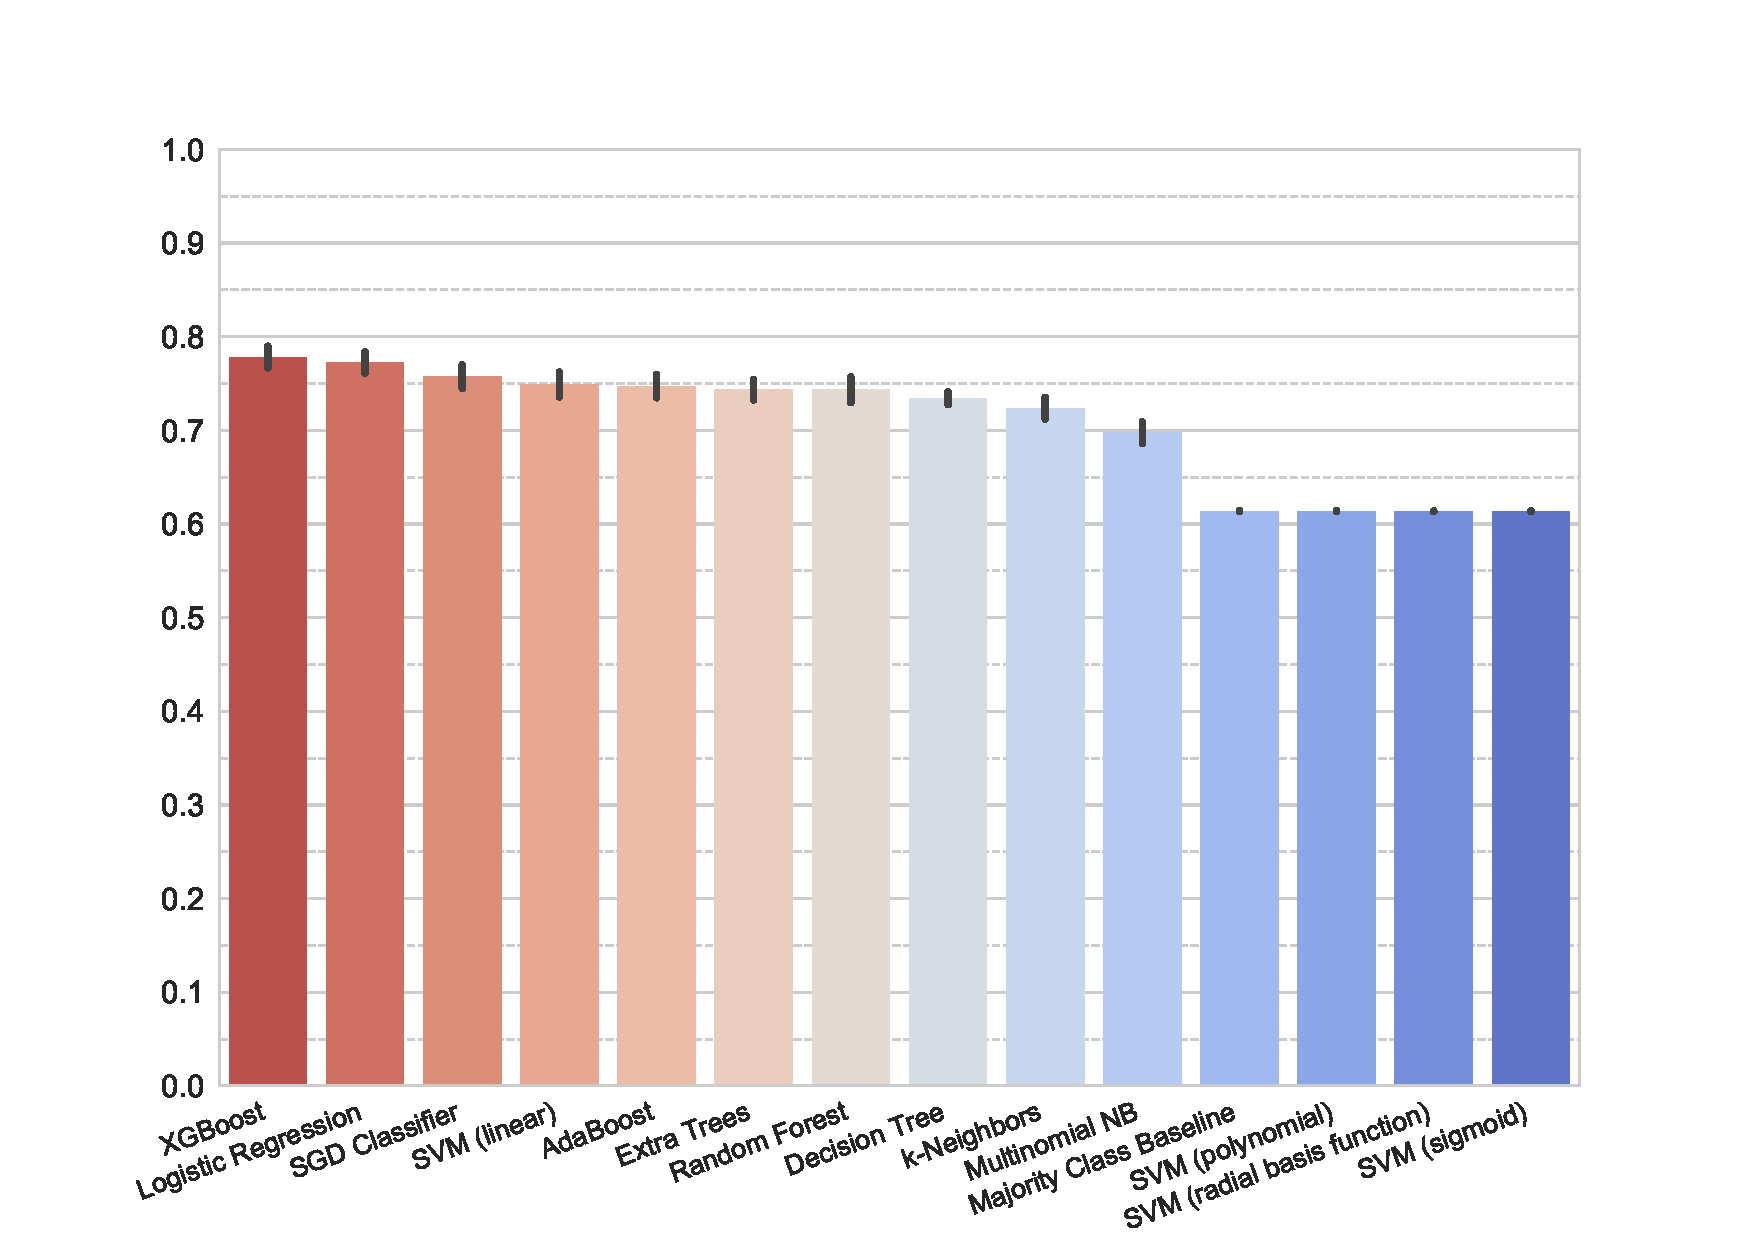
\includegraphics[width=0.8\linewidth]{images/classifier}
\end{figure}

To find the best performing classification algorithms, thirten (see table \ref{tbl:algo}) were selected and compared. Except \emph{XGBoost}\footnote{XGBoost is not part of scikit-learn. The implementation presented in \cite{DBLP:journals/corr/ChenG16} was used.} and \emph{Extra Trees Classifier}, all algorithms were used in at least one paper presented in section \ref{sec:argmine}. The binary unigram vector computed on the whole sentence was used as the only feature. Stratified k-fold with k equals five was used to assess the quality of the algorithm.





%\begin{table}[h]
%\centering
%\label{tbl:algo}
%\caption{All evaluated classification algorithms. The F1 score shows the classification performance with the unigram feature.}
%\begin{tabularx}{\textwidth}{XlX}
%\toprule
%Algorithm & F1 Score & Used in\\ \midrule
%
%XGBoost & 0.76 & -\\ 
%
%Logistic Regression & 0.75 &  \cite{Dusmanu2017Argument-Mining,Daxenberger2017What-is-the-EssAker2017What-works-and-,Lippi2016Argumentation-M}\\ 
%
%AdaBoost & 0.74 &  \cite{Aker2017What-works-and-}\\  
%
%Linear SVC & 0.73 & \cite{Aker2017What-works-and-}\\  
%
%Decision Tree & 0.72 &  \cite{Stab2014Identifying-Arg,Lippi2016Argumentation-M}\\ 
%
%Stochastic Gradient Descent & 0.72 & -\\ 
%
%
%Random Forest & 0.72 &  \cite{Dusmanu2017Argument-Mining,Stab2014Identifying-Arg,Eckle-Kohler2015On-the-Role-of-,Aker2017What-works-and-,Lippi2016Argumentation-M}\\  
%
%Extra Trees Classifier & 0.72 & - \\
%
%K Neighbors & 0.72 &  \cite{Aker2017What-works-and-}\\ 
%
%
%Support Vector Machine (non-linear kernel) & 0.60 & \cite{Stab2014Identifying-Arg,Eckle-Kohler2015On-the-Role-of-,Park:2012:ICC:2391171.2391173,Lippi2016Argumentation-M,Habernal2016Argumentation-M}\\ 
%
%
%Naive Bayes & 0.60 & \cite{Stab2014Identifying-Arg,Eckle-Kohler2015On-the-Role-of-,Aker2017What-works-and-,Park:2012:ICC:2391171.2391173,Lippi2016Argumentation-M}\\  
%
%
% \bottomrule 
%\end{tabularx}
%
%\end{table}


Tree-based methods and linear models work good. Support Vector Machines with non-linear kernels assigne \texttt{NONE} to all sentences.

As XGBoost and Logistic Regression already work in a pleasing way, no further investigations on the performance of other algorithms were done. A set of hyper-parameters for XGBoost were tested using exhaustive grid search and randomized search. However, no significant increase in the F1 score could be achieved.

In the following sections, all experiments were done using XGBoost (1000 estimators).


\section{Preprocessing}
In addition to the full sentence, preprocessed versions of it were used in the feature calculation.

Different parts of the sentence were used. The \emph{first part} contains all words from the beginning of the sentence to the first object, while the \emph{last part} contains all words from the second object to the end of the sentence. The \emph{middle part} contains all words between the first and the second object.

Another processing step was done to assess how important the objects are for the classification. The objects either stayed untouched, were removed or replaced. Two different replacement strategies were tested. First, both objects were replaced by the term \emph{OBJECT} (replacement). Second, the first object was replaced by \emph{OBJECT\_A} and the second by \emph{OBJECT\_B} (distinct replacement). Some examples are shown in table \ref{preprocessing_example}.

\begin{table}[h]
\centering

\caption{Preprocessing examples for the sentence \enquote{\emph{In my mind, Python is better than Ruby}}}
\label{preprocessing_example}
\begin{tabularx}{\linewidth}{lX}
\toprule
Preprocessing & Result \\ \midrule
Middle part & Python is better than Ruby \\
Middle part, removal & is better than \\
Full sentence, distinct replacement &In my mind, OBJECT\_A is better than OBJECT\_B \\
First part, removal & In my mind, \\
\bottomrule
\end{tabularx}

\end{table}


\section{Features}


\section{Experiments}
\subsection{Baselines}
\label{sec:3_baseline}
As described in section \ref{sec:argmine}, there is no task which is similar enough to this one which could be used as a baseline. Thus, two baselines using the obtained data were created. The first baseline, shown in table \ref{tbl:3stratifiedbaseline}, assigns all sentences to the class \texttt{NONE}.

% 24.3
\begin{table}[!htb]
    \begin{minipage}{.5\linewidth}
      \caption{Random (stratified) baseline for the classification task.}
      \label{tbl:3stratifiedbaseline}
      \centering
      
\begin{tabular}{@{}lrrrr@{}}
\toprule
 	&	 precision &	 recall &	 f1 score  \\ \midrule 
\texttt{BETTER}	&	 0.22 \scriptsize{(0.02)} &	 0.23 \scriptsize{(0.02)} &	 0.22 \scriptsize{(0.02)}  \\ 
\texttt{WORSE}	&	 0.10 \scriptsize{(0.02)} &	 0.08 \scriptsize{(0.02)} &	 0.09 \scriptsize{(0.02)}  \\ 
\texttt{NONE}	&	 0.74 \scriptsize{(0.01)} &	 0.74 \scriptsize{(0.01)} &	 0.74 \scriptsize{(0.01)}  \\ 
average	&	 0.59 \scriptsize{(0.01)} &	 0.59 \scriptsize{(0.01)} &	 0.59 \scriptsize{(0.01)}  \\ 
\bottomrule
\end{tabular} 

  \end{minipage}%
    \begin{minipage}{.5\linewidth}
      \centering
        \caption{Majority class baseline for the classification task.}
        \label{tbl:3majoritybaseline}
\begin{tabular}{@{}lrrrr@{}}
\toprule
 	&	 precision &	 recall &	 f1 score  \\ \midrule 
\texttt{BETTER}	&	 0.00 \scriptsize{(0.00)} &	 0.00 \scriptsize{(0.00)} &	 0.00 \scriptsize{(0.00)}  \\ 
\texttt{WORSE}	&	 0.00 \scriptsize{(0.00)} &	 0.00 \scriptsize{(0.00)} &	 0.00 \scriptsize{(0.00)}  \\ 
\texttt{NONE}	&	 0.73 \scriptsize{(0.00)} &	 1.00 \scriptsize{(0.00)} &	 0.84 \scriptsize{(0.00)}  \\ 
average	&	 0.53 \scriptsize{(0.00)} &	 0.73 \scriptsize{(0.00)} &	 \textbf{0.61} \scriptsize{(0.00)}  \\ 
\bottomrule
\end{tabular}
    \end{minipage} 
\end{table}



The second baseline is created by assigning classes to the data at random, respecting the distribution of classes in the original data. The results are shown in table \ref{tbl:3majoritybaseline}.

% 24.3
The baselines for the binary classification task are shown in tables \ref{tbl:binmaj} and \ref{tbl:binstrat}.


\begin{table}[!htb]
    \begin{minipage}{.5\linewidth}
      \caption{Random (stratified) baseline for the binary classification task.}
      \label{tbl:binmaj}
      \centering
      
\begin{tabular}{@{}lrrrr@{}}
\toprule
 	&	 precision &	 recall &	 f1 score  \\ \midrule 
\texttt{ARG}	&	 0.31 \scriptsize{(0.02)} &	 0.31 \scriptsize{(0.02)} &	 0.31 \scriptsize{(0.02)}  \\ 
\texttt{NONE}	&	 0.74 \scriptsize{(0.01)} &	 0.74 \scriptsize{(0.01)} &	 0.74 \scriptsize{(0.01)}  \\ 
average	&	 0.62 \scriptsize{(0.01)} &	 0.62 \scriptsize{(0.01)} &	 \textbf{0.62} \scriptsize{(0.01)}  \\ 
\bottomrule
\end{tabular}

  \end{minipage}%
    \begin{minipage}{.5\linewidth}
      \centering
        \caption{Majority class baseline for the binary classification task.}
        \label{tbl:binstrat}
\begin{tabular}{@{}lrrrr@{}}
\toprule
 	&	 precision &	 recall &	 f1 score  \\ \midrule 
\texttt{ARG}	&	 0.00 \scriptsize{(0.00)} &	 0.00 \scriptsize{(0.00)} &	 0.00 \scriptsize{(0.00)}  \\ 
\texttt{NONE}	&	 0.73 \scriptsize{(0.00)} &	 1.00 \scriptsize{(0.00)} &	 0.84 \scriptsize{(0.00)}  \\ 
average	&	 0.53 \scriptsize{(0.00)} &	 0.73 \scriptsize{(0.00)} &	 0.61 \scriptsize{(0.00)}  \\ 
\bottomrule
\end{tabular}
    \end{minipage} 
\end{table}


For all baselines, the scikit-learn's \texttt{DummyClassifer} was used.


\subsection{Results}
\label{sec:3_results}
The classification results are presented in the tables below. Every table shows the best out of five folds. The standard derivation is stated in brackets. Top results are printed in bold. Only the best feature configurations are shown.

Tables \ref{tbl:se3} to \ref{tbl:ngram_3} show the results of different vector representations of the sentence. Simple unigrams and the more complex sentence embeddings yield almost the same performance. The main difference is with the class \texttt{WORSE}.


\begin{figure}[h]
      \caption{F1 score for the three-class scenario.} 
    \label{tbl:3_conf_inf}
 \centering
	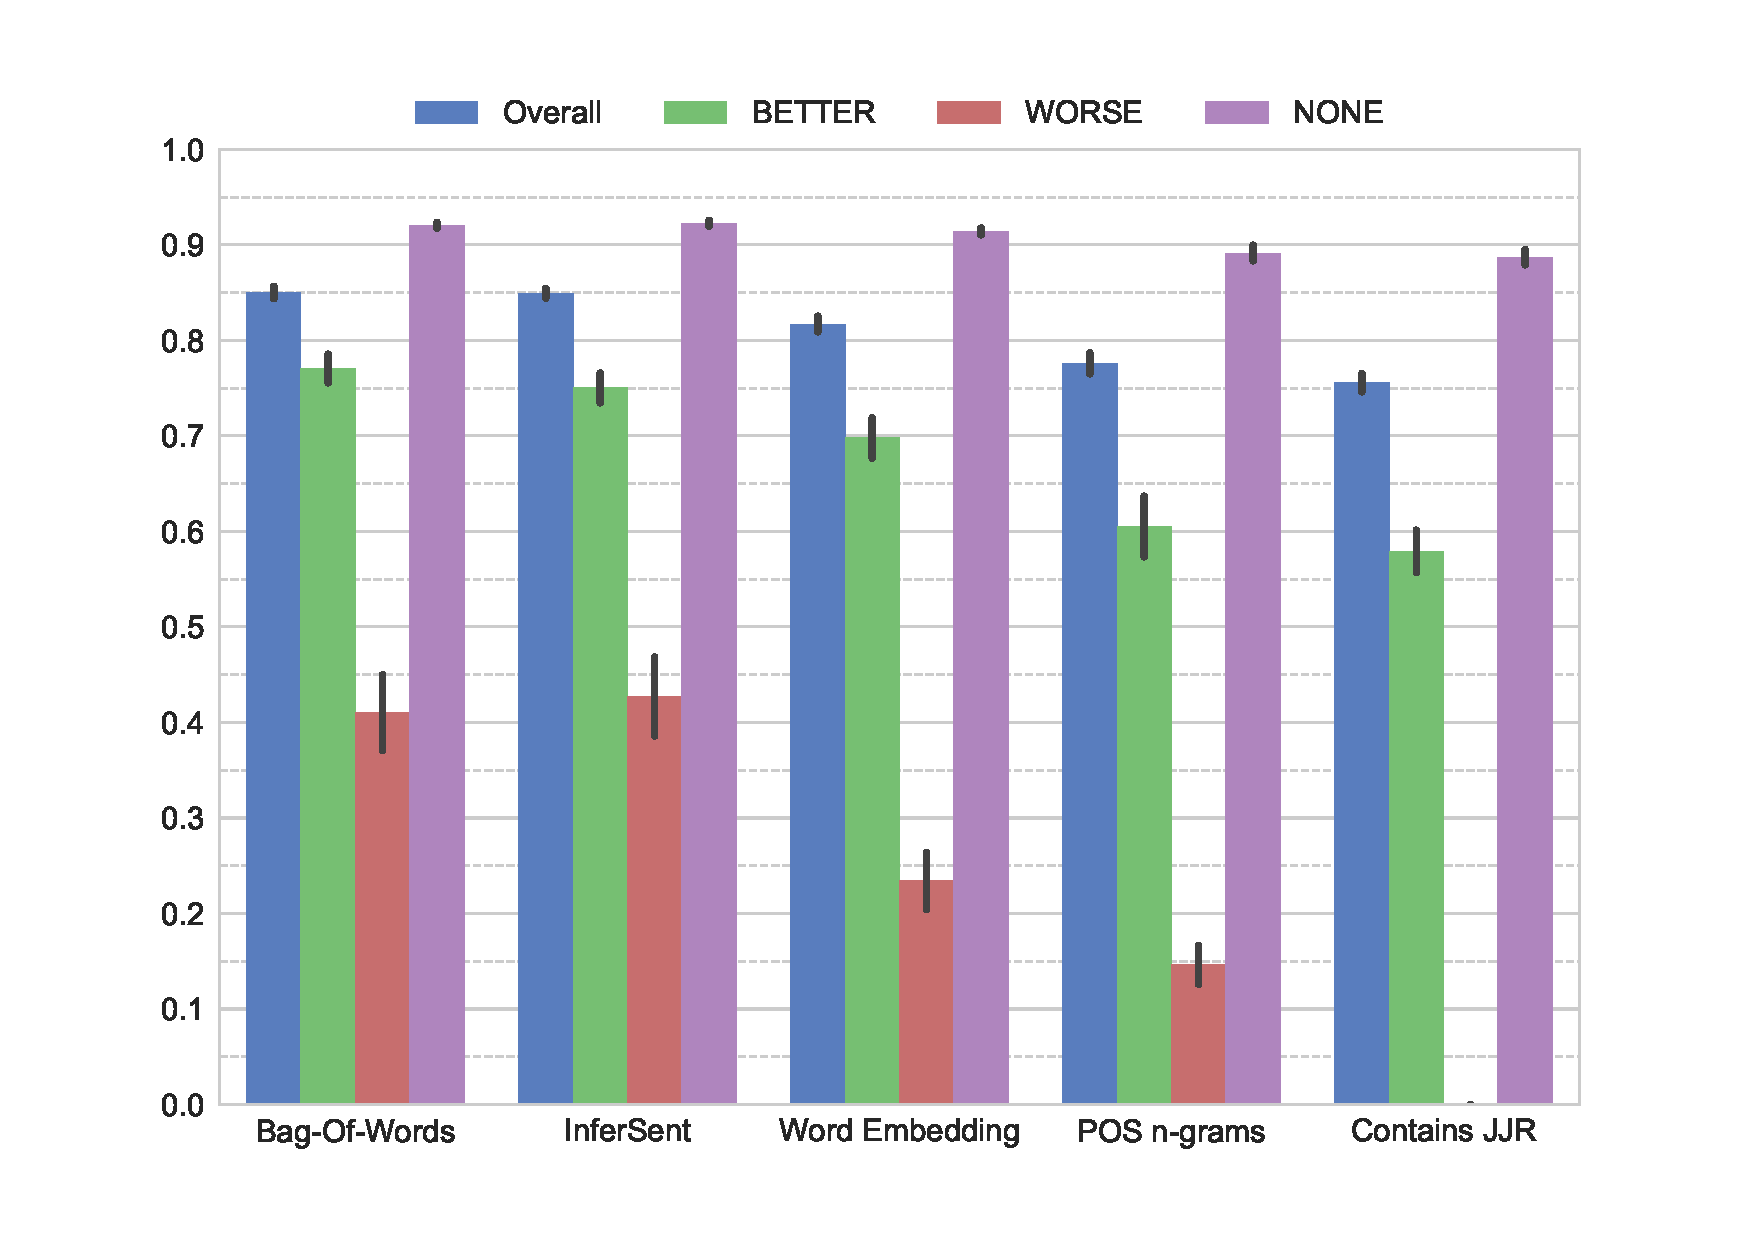
\includegraphics[width=0.8\textwidth]{images/experiments/f1-False}

\end{figure}

%\begin{table}[h]
%    \begin{minipage}{.5\linewidth}
%    
%        \caption{\emph{Sentence embeddings on the middle part of the sentence}. (Standard derivation)} 
%        \label{tbl:se3}
% 4.4
%\begin{tabular}{@{}lrrrr@{}}
%\toprule
% 	&	 precision &	 recall &	 f1 score  \\ \midrule 
%BETTER	&	 0.81 \scriptsize{(0.04)} &	 0.79 \scriptsize{(0.02)} &	 0.80 \scriptsize{(0.03)}  \\ 
%WORSE	&	 0.57 \scriptsize{(0.04)} &	 0.33 \scriptsize{(0.05)} &	 0.42 \scriptsize{(0.04)}  \\ 
%NONE	&	 0.91 \scriptsize{(0.01)} &	 0.96 \scriptsize{(0.01)} &	 0.93 \scriptsize{(0.01)}  \\ 
%average	&	 0.86 \scriptsize{(0.01)} &	 0.87 \scriptsize{(0.01)} &	 0.86 \scriptsize{(0.01)}  \\ 
%\bottomrule
%\end{tabular}
%  \end{minipage} \hfill
%    \begin{minipage}{.5\linewidth}
%    \caption{ \emph{Binary unigram vector} for all unigrams in the middle part of the sentence. } 
%         % 4.4
%         \begin{tabular}{@{}lrrrr@{}}
%\toprule
% 	&	 precision &	 recall &	 f1 score  \\ \midrule 
%BETTER	&	 0.82 \scriptsize{(0.03)} &	 0.79 \scriptsize{(0.04)} &	 0.81 \scriptsize{(0.03)}  \\ 
%WORSE	&	 0.71 \scriptsize{(0.06)} &	 0.23 \scriptsize{(0.02)} &	 0.35 \scriptsize{(0.02)}  \\ 
%NONE	&	 0.89 \scriptsize{(0.01)} &	 0.97 \scriptsize{(0.01)} &	 0.93 \scriptsize{(0.01)}  \\ 
%average	&	 0.86 \scriptsize{(0.01)} &	 0.87 \scriptsize{(0.01)} &	 0.86 \scriptsize{(0.01)}  \\ 
%\bottomrule
%\end{tabular}
%    \end{minipage} 
%\end{table}




Mean Word Embeddings (table \ref{tbl:3_mwe}) and POS n-grams (table \ref{tbl:ngram_3}) are barely able to recognize \texttt{WORSE} at all.

%\begin{table}[h]
%    \begin{minipage}{.5\linewidth}
%   \caption{ \emph{Mean Word Embeddings} for the middle part of the sentence. } 
%    \label{tbl:3_mwe}
%\begin{tabular}{@{}lrrrr@{}}
%\toprule
% 	&	 precision &	 recall &	 f1 score  \\ \midrule 
%\texttt{BETTER}	&	 0.70 \scriptsize{(0.01)} &	 0.75 \scriptsize{(0.04)} &	 0.72 \scriptsize{(0.02)}  \\ 
%\texttt{WORSE}	&	 0.44 \scriptsize{(0.16)} &	 0.04 \scriptsize{(0.04)} &	 0.08 \scriptsize{(0.07)}  \\ 
%\texttt{NONE}	&	 0.88 \scriptsize{(0.01)} &	 0.96 \scriptsize{(0.01)} &	 0.92 \scriptsize{(0.00)}  \\ 
%average	&	 0.81 \scriptsize{(0.01)} &	 0.84 \scriptsize{(0.01)} &	 0.81 \scriptsize{(0.01)}  \\ 
%\bottomrule
%\end{tabular}
%  \end{minipage} \hfill
%    \begin{minipage}{.5\linewidth}
%  
%     \caption{500 most frequent \emph{part-of-speech bi-, tri- and four-grams}; weighted by tf-idf.} 
%       \label{tbl:ngram_3}
%\begin{tabular}{@{}lrrrr@{}}
%\toprule
% 	&	 precision &	 recall &	 f1 score  \\ \midrule 
%\texttt{BETTER}	&	 0.63 \scriptsize{(0.04)} &	 0.67 \scriptsize{(0.05)} &	 0.65 \scriptsize{(0.04)}  \\ 
%\texttt{WORSE}	&	 0.64 \scriptsize{(0.19)} &	 0.07 \scriptsize{(0.02)} &	 0.13 \scriptsize{(0.04)}  \\ 
%\texttt{NONE}	&	 0.87 \scriptsize{(0.01)} &	 0.94 \scriptsize{(0.01)} &	 0.90 \scriptsize{(0.01)}  \\ 
%average	&	 0.80 \scriptsize{(0.03)} &	 0.82 \scriptsize{(0.01)} &	 0.79 \scriptsize{(0.01)}  \\ 
%\bottomrule
%\end{tabular}
%    \end{minipage} 
%\end{table}


The boolean feature (table \ref{tbl:3jjr}) can yield an f1 score fiften points higher than the majority class baseline. However, it does not recognize any sentences of the class \texttt{WORSE}.

%\begin{table}[h] 
% \centering 
% \caption{Boolean feature, capturing the appearance of the part-of-speech JJR in the middle part of the sentence.} 
% \label{tbl:3jjr}
%\begin{tabular}{@{}lrrrr@{}}
%\toprule
% 	&	 precision &	 recall &	 f1 score  \\ \midrule 
%\texttt{BETTER}	&	 0.60 \scriptsize{(0.02)} &	 0.58 \scriptsize{(0.02)} &	 0.59 \scriptsize{(0.02)}  \\ 
%\texttt{WORSE}	&	 0.00 \scriptsize{(0.00)} &	 0.00 \scriptsize{(0.00)} &	 0.00 \scriptsize{(0.00)}  \\ 
%\texttt{NONE}	&	 0.84 \scriptsize{(0.01)} &	 0.94 \scriptsize{(0.01)} &	 0.89 \scriptsize{(0.01)}  \\ 
%average	&	 0.73 \scriptsize{(0.01)} &	 0.80 \scriptsize{(0.01)} &	 0.76 \scriptsize{(0.01)}  \\ 
%\bottomrule
%\end{tabular}
%\end{table}



\begin{figure}[h]
    \begin{minipage}{.5\textwidth}
   \caption{Precision for the three-classes scenario.} 
    \label{tbl:3_conf_inf}
 \centering
 \hspace*{-1cm}
	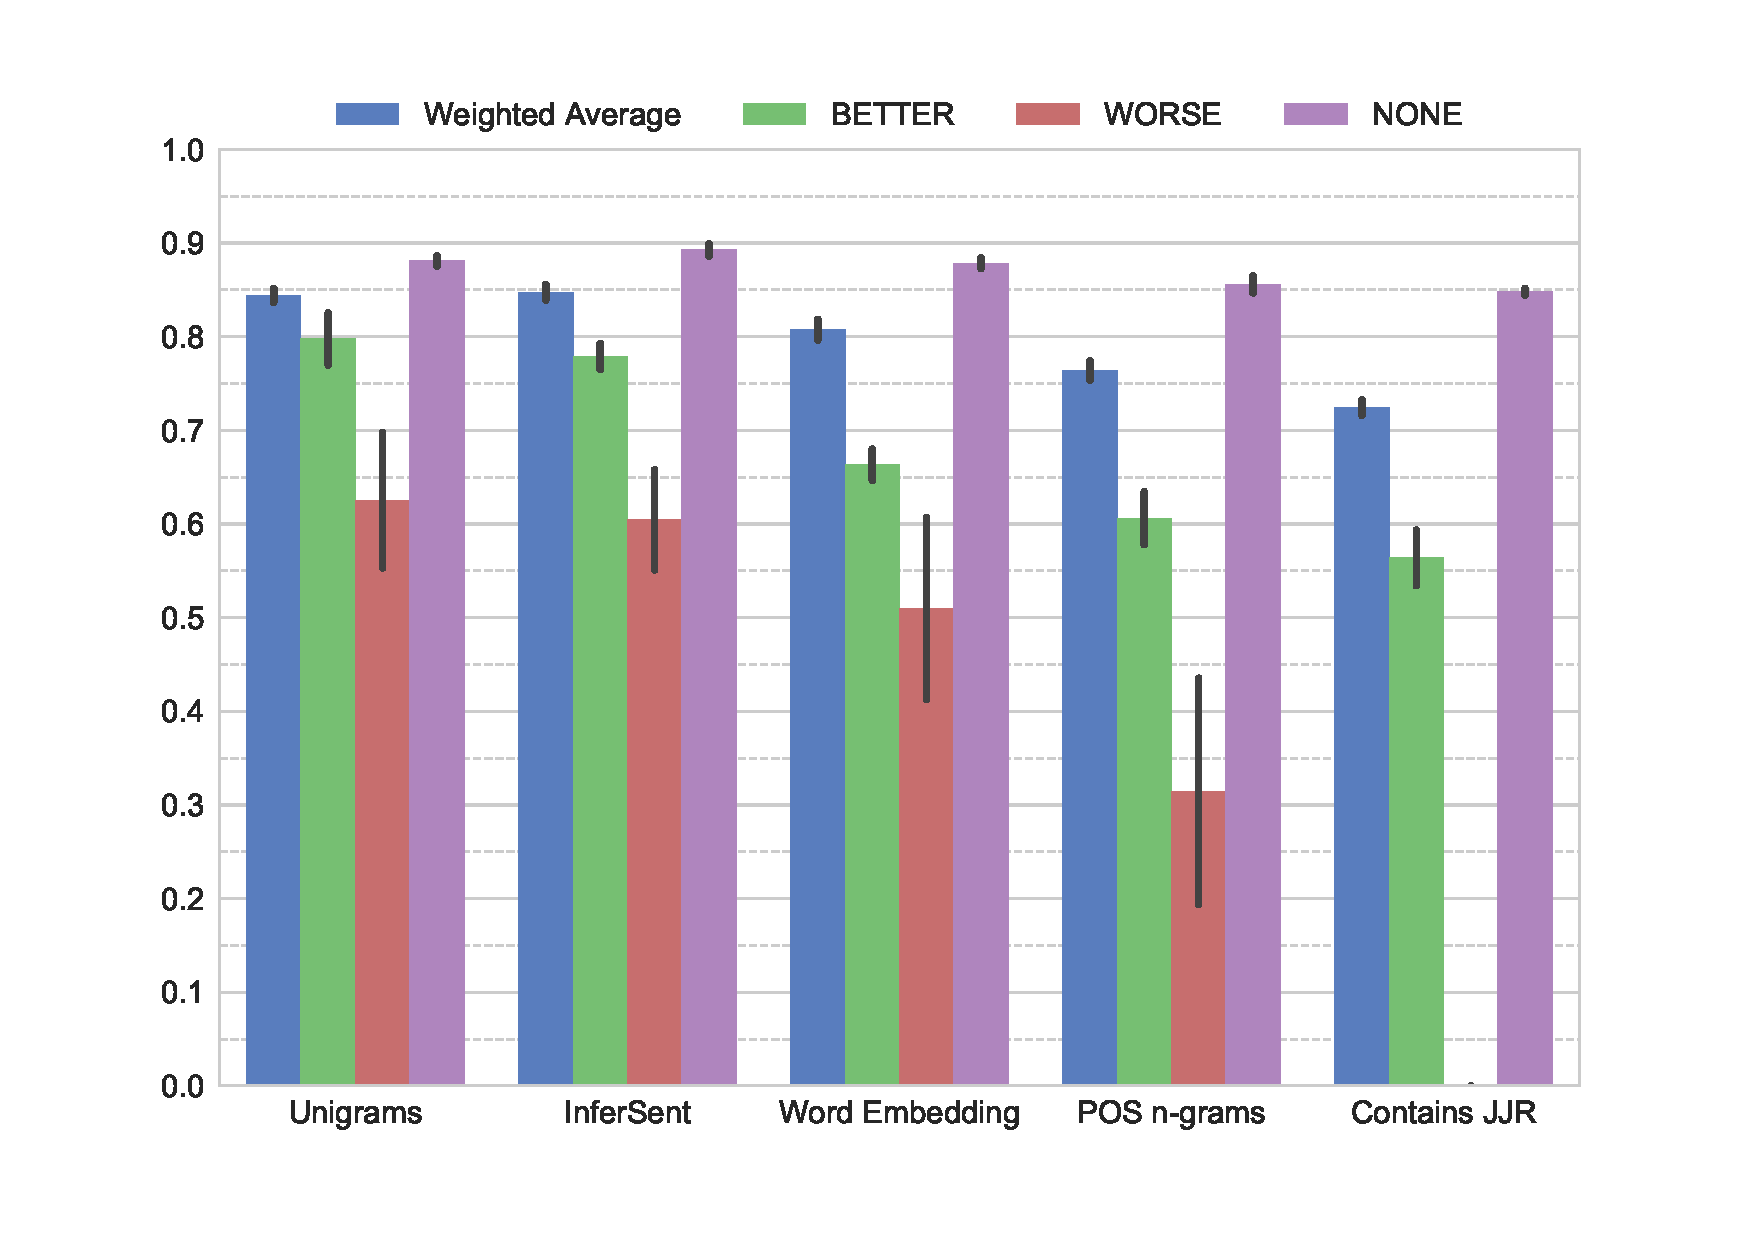
\includegraphics[width=1.25\textwidth]{images/experiments/precision-False}
  \end{minipage} \hfill
    \begin{minipage}{.5\textwidth}
   \hspace*{+1cm}
     \caption{Recall for the three-classes scenario.} 
       \label{tbl:3_conf_uni}
 \centering
	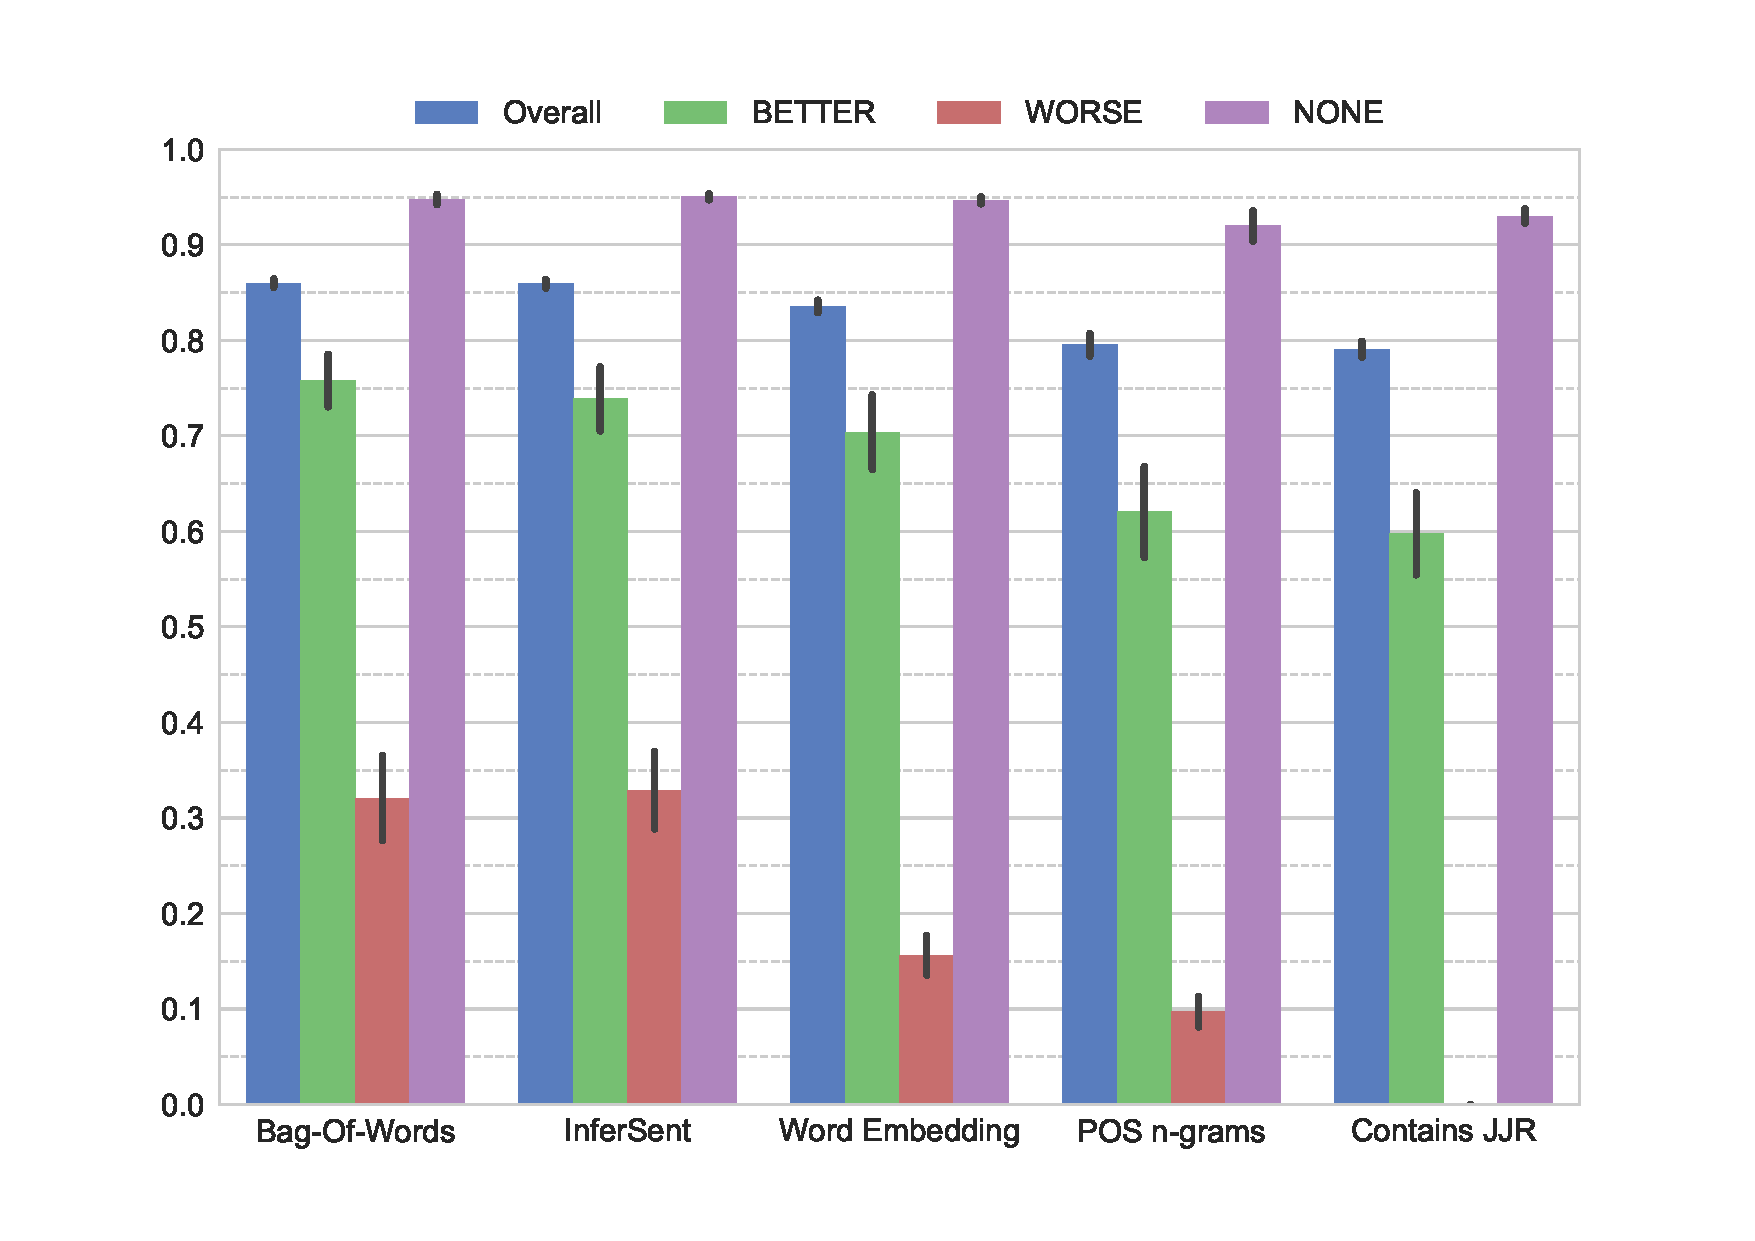
\includegraphics[width=1.25\textwidth]{images/experiments/recall-False}
    \end{minipage} 
\end{figure}

Using only the middle part of the sentence increased the f1 score by five to seven points every time. The removal or replacement of the object only altered the f1 score by about 0.01 points, which is equal to the standard derivation.




% === binary 
Tables \ref{tbl:2_infer} to \ref{tbl:2_jjr} show the results for the binary classification.



\begin{figure}[h]
      \caption{F1 score for the binary scenario.} 
    \label{tbl:3_conf_inf}
 \centering
	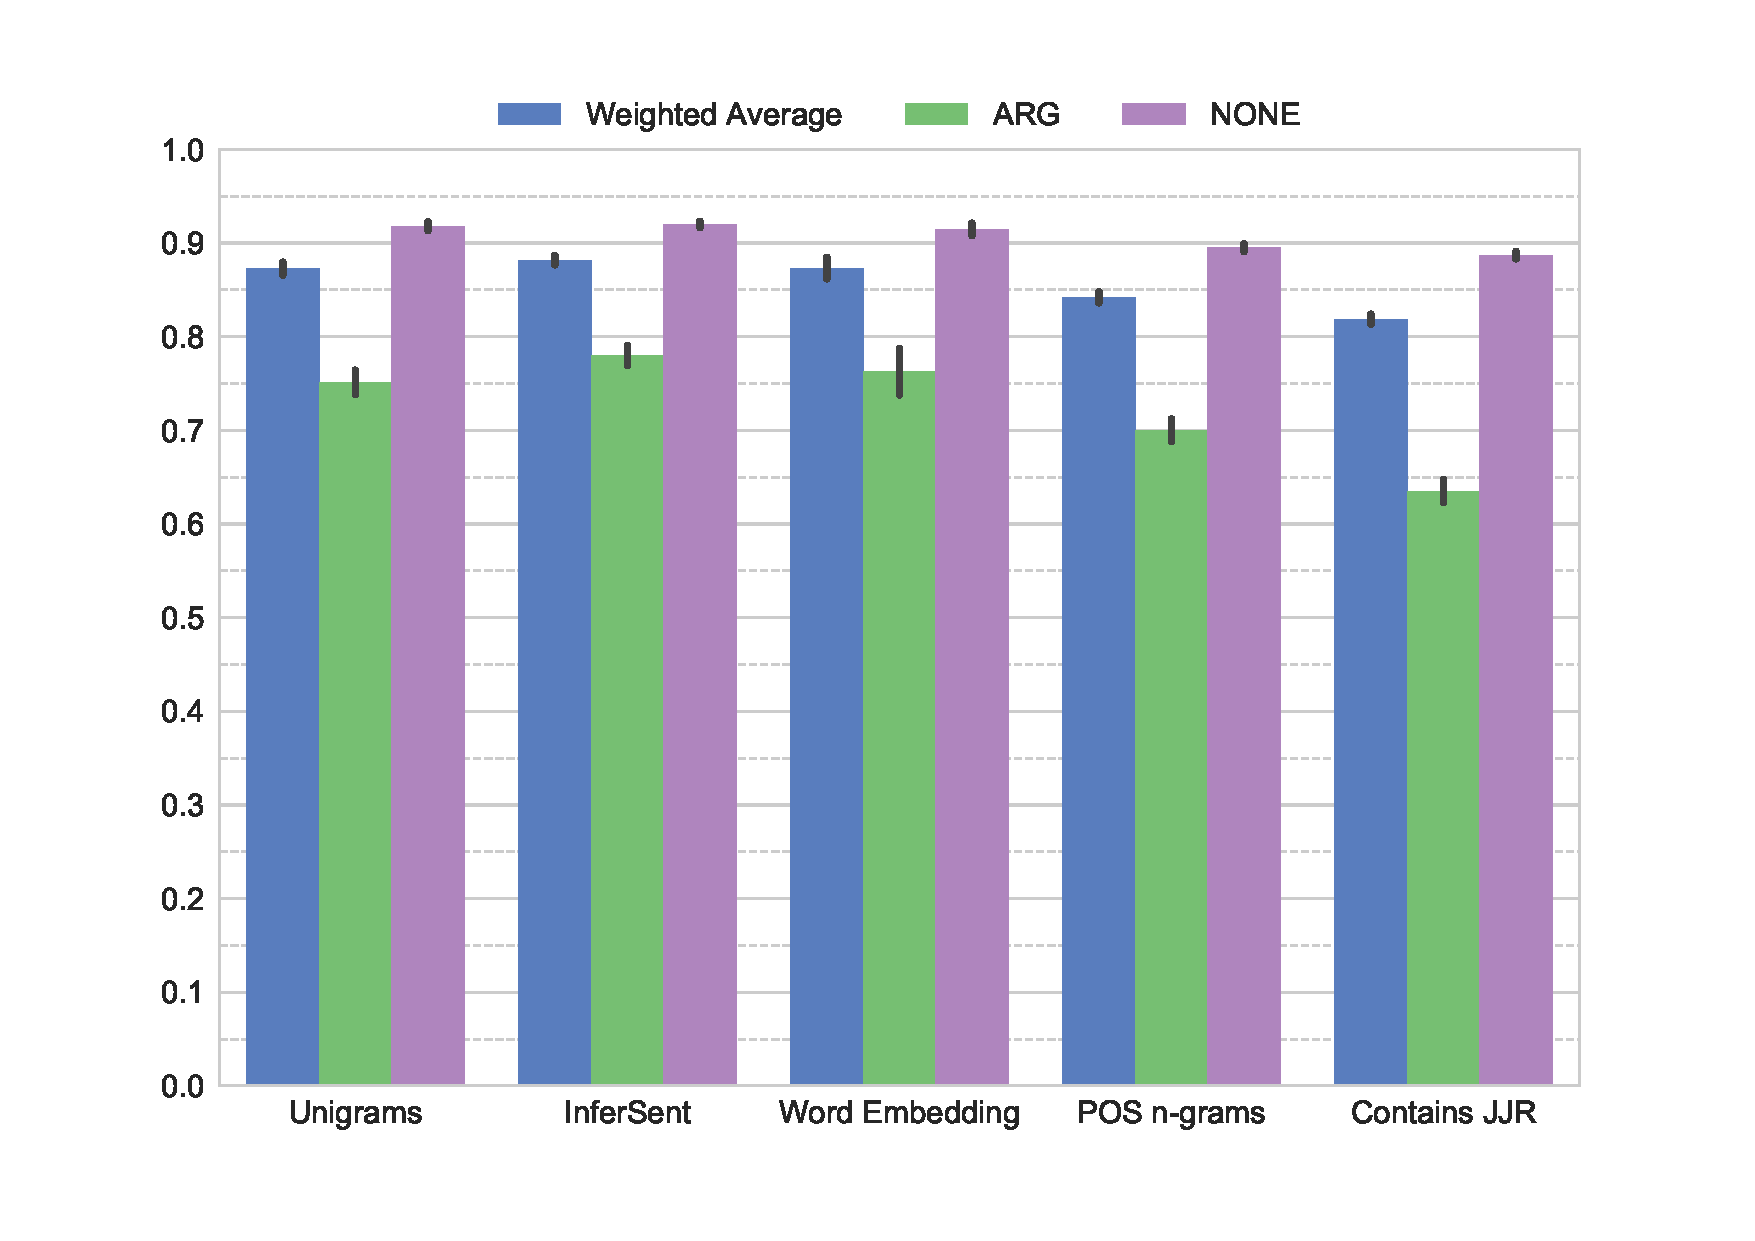
\includegraphics[width=0.8\textwidth]{images/experiments/f1-True}

\end{figure}

%\begin{table}[!htb]
%    \begin{minipage}{.5\linewidth}
%      \caption{infersent}
%      \label{tbl:2_infer}
%      \centering
%      
%\begin{tabular}{@{}lrrrr@{}}
%\toprule
% 	&	 precision &	 recall &	 f1 score  \\ \midrule
%ARG	&	 0.80 \scriptsize{(0.01)} &	 0.82 \scriptsize{(0.04)} &	 0.81 \scriptsize{(0.02)}  \\
%NONE	&	 0.93 \scriptsize{(0.01)} &	 0.92 \scriptsize{(0.01)} &	 0.93 \scriptsize{(0.01)}  \\
%average	&	 0.90 \scriptsize{(0.01)} &	 0.89 \scriptsize{(0.01)} &	 0.89 \scriptsize{(0.01)}  \\
%\bottomrule
%\end{tabular}
%
%  \end{minipage}%
%    \begin{minipage}{.5\linewidth}
%      \centering
%        \caption{unigrams}
%        \label{tbl:2_uni}
%\begin{tabular}{@{}lrrrr@{}}
%\toprule
% 	&	 precision &	 recall &	 f1 score  \\ \midrule 
%ARG	&	 0.84 \scriptsize{(0.02)} &	 0.75 \scriptsize{(0.04)} &	 0.79 \scriptsize{(0.03)}  \\ 
%NONE	&	 0.91 \scriptsize{(0.01)} &	 0.95 \scriptsize{(0.01)} &	 0.93 \scriptsize{(0.01)}  \\ 
%average	&	 0.89 \scriptsize{(0.01)} &	 0.89 \scriptsize{(0.01)} &	 0.89 \scriptsize{(0.01)}  \\ 
%\bottomrule
%\end{tabular}
%    \end{minipage} 
%\end{table}
%
%
%
%\begin{table}[!htb]
%    \begin{minipage}{.5\linewidth}
%      \caption{2 mwe}
%      \label{tbl:2_mwe}
%      \centering
%      
%\begin{tabular}{@{}lrrrr@{}}
%\toprule
% 	&	 precision &	 recall &	 f1 score  \\ \midrule
%ARG	&	 0.77 \scriptsize{(0.01)} &	 0.80 \scriptsize{(0.04)} &	 0.79 \scriptsize{(0.02)}  \\
%NONE	&	 0.93 \scriptsize{(0.01)} &	 0.91 \scriptsize{(0.01)} &	 0.92 \scriptsize{(0.01)}  \\
%average	&	 0.88 \scriptsize{(0.01)} &	 0.88 \scriptsize{(0.01)} &	 0.88 \scriptsize{(0.01)}  \\
%\bottomrule
%\end{tabular}
%  \end{minipage}%
%    \begin{minipage}{.5\linewidth}
%      \centering
%        \caption{pos}
%        \label{tbl:2_uni}
%\begin{tabular}{@{}lrrrr@{}}
%\toprule
% 	&	 precision &	 recall &	 f1 score  \\ \midrule
%ARG	&	 0.77 \scriptsize{(0.01)} &	 0.68 \scriptsize{(0.04)} &	 0.72 \scriptsize{(0.03)}  \\
%NONE	&	 0.89 \scriptsize{(0.01)} &	 0.92 \scriptsize{(0.01)} &	 0.91 \scriptsize{(0.01)}  \\
%average	&	 0.86 \scriptsize{(0.01)} &	 0.86 \scriptsize{(0.01)} &	 0.86 \scriptsize{(0.01)}  \\
%\bottomrule
%\end{tabular}
%    \end{minipage} 
%\end{table}
%
%\begin{table}[h]
% \centering
% \caption{ Contains JJR ('middle part', ExtractMiddlePart(processing=None)) }
% \label{tbl:2_jjr}
%\begin{tabular}{@{}lrrrr@{}}
%\toprule
% 	&	 precision &	 recall &	 f1 score  \\ \midrule
%ARG	&	 0.75 \scriptsize{(0.01)} &	 0.54 \scriptsize{(0.01)} &	 0.63 \scriptsize{(0.01)}  \\
%NONE	&	 0.85 \scriptsize{(0.00)} &	 0.93 \scriptsize{(0.00)} &	 0.89 \scriptsize{(0.00)}  \\
%average	&	 0.82 \scriptsize{(0.00)} &	 0.83 \scriptsize{(0.00)} &	 0.82 \scriptsize{(0.00)}  \\
%\bottomrule
%\end{tabular}
%\end{table}

As in section \ref{sec:3_results}, sentence embedding and the unigram feature performed best and got equal results. In contrast to the three-classes scenario, they are closely followed by mean word embeddings. In summary, all vector representations worked good and got f1 scores close to each other. The feature capturing the appearance of comparative adjectives is again the worst, yet the score is nineten points above the baseline.



\begin{figure}[h]
    \begin{minipage}{.5\linewidth}
   \caption{Precision for the binary scenario.} 
    \label{tbl:3_conf_inf}
 \centering
	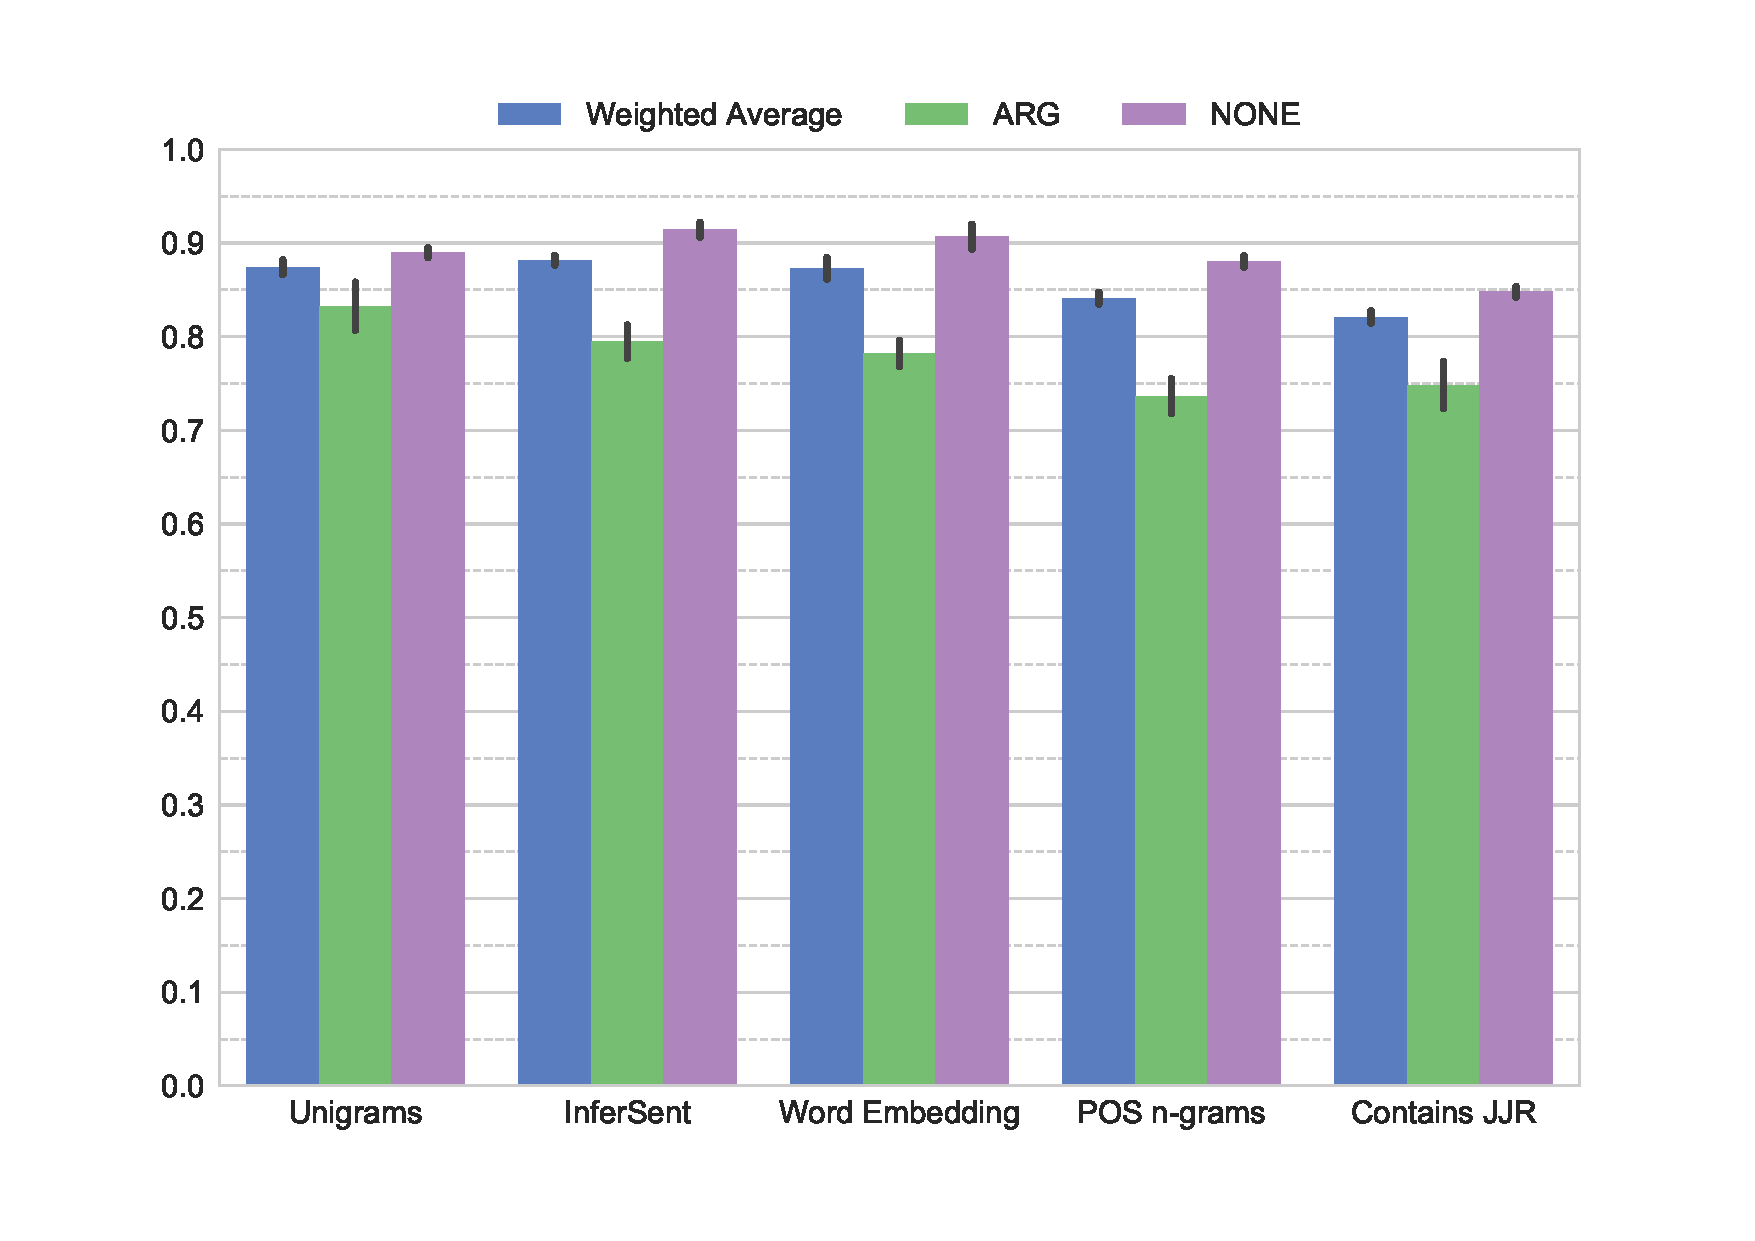
\includegraphics[width=1\linewidth]{images/experiments/precision-True}
  \end{minipage} 
    \begin{minipage}{.5\linewidth}
  
     \caption{Recall for the binary scenario.} 
       \label{tbl:3_conf_uni}
 \centering
	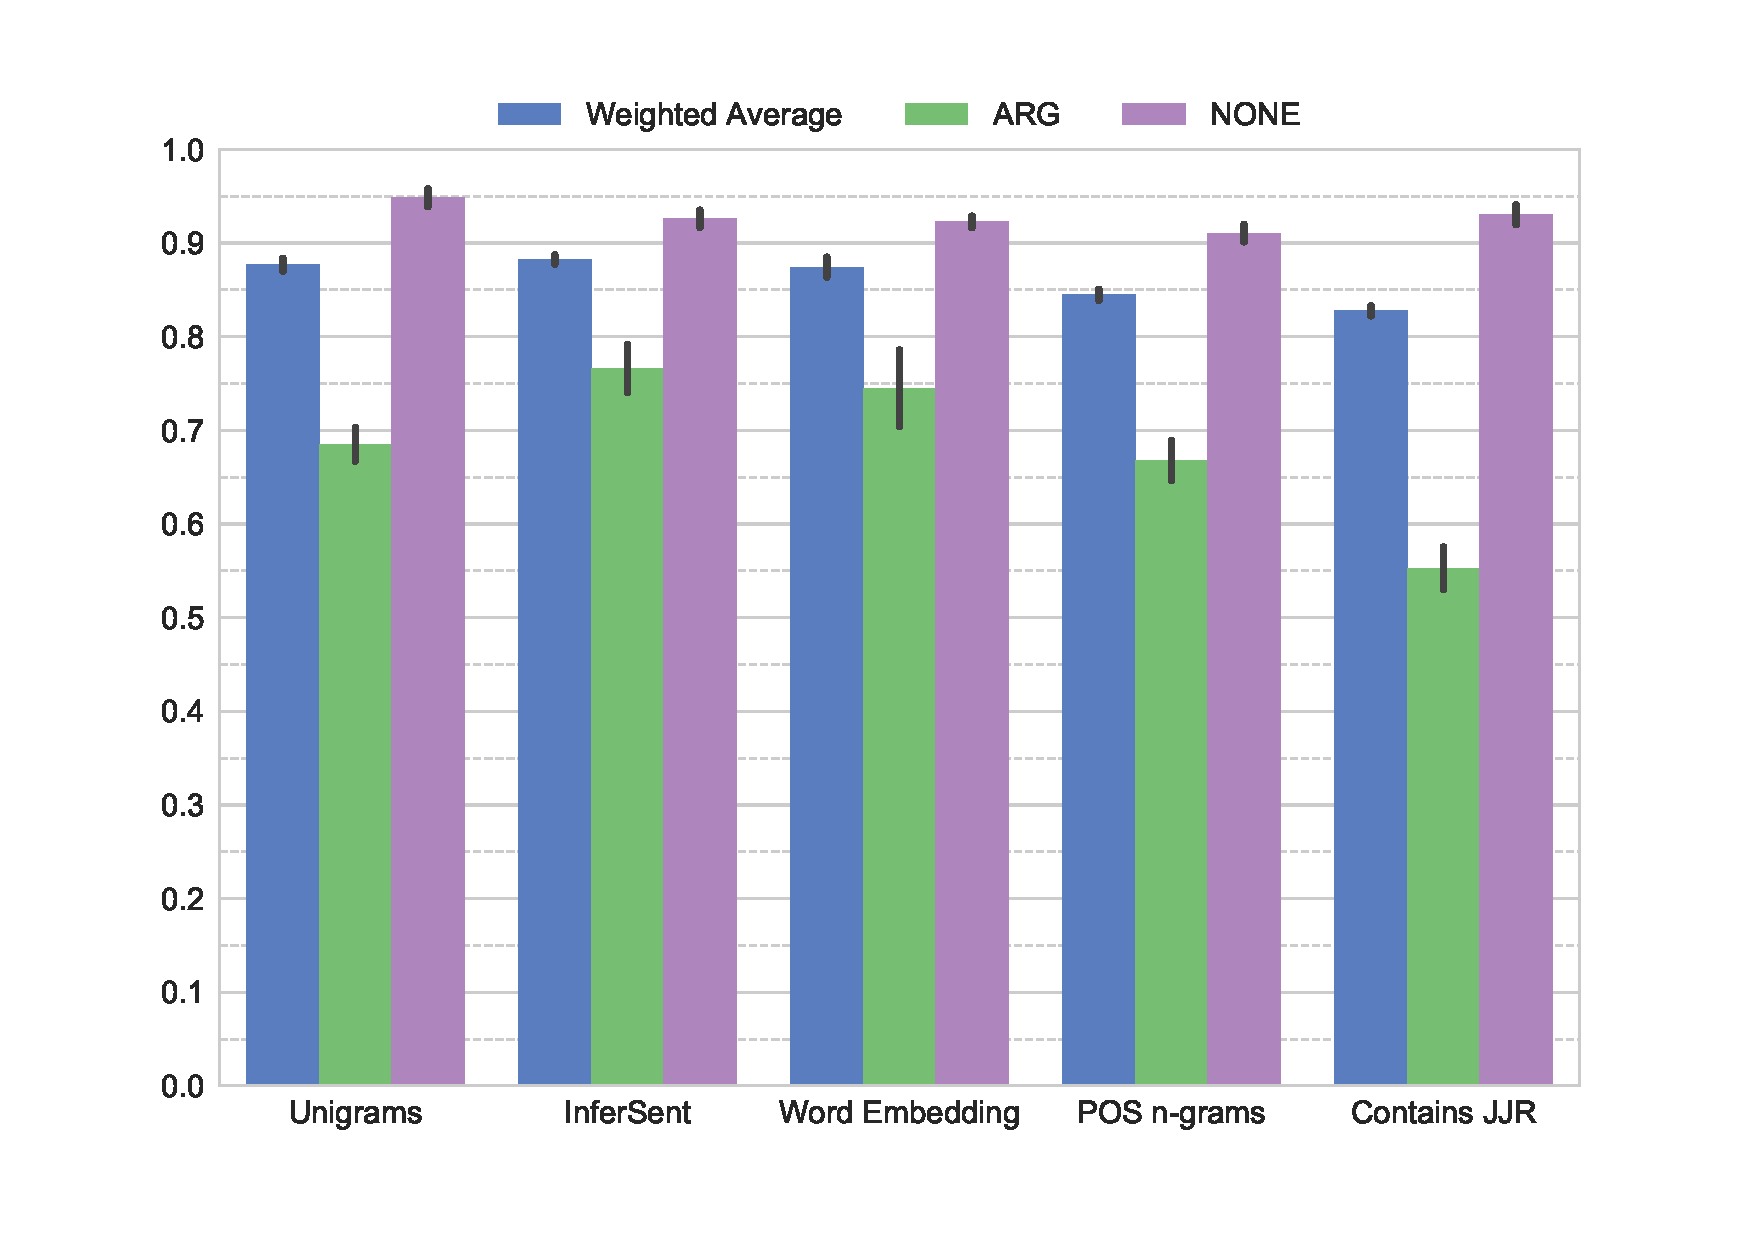
\includegraphics[width=1\linewidth]{images/experiments/recall-True}
    \end{minipage} 
\end{figure}



\subsection{Error analysis}

The tables \ref{tbl:3_conf_inf} and \ref{tbl:3_conf_uni} display the confusion matrices for the two best features in the three-label scenario (sentence embeddings and unigrams). The confusion matrices of each fold per feature were added to create these tables.





\begin{figure}[h]
    \begin{minipage}{.5\linewidth}
   \caption{Confusion matrix for the sentence embedding feature} 
    \label{tbl:3_conf_inf}
 \centering
	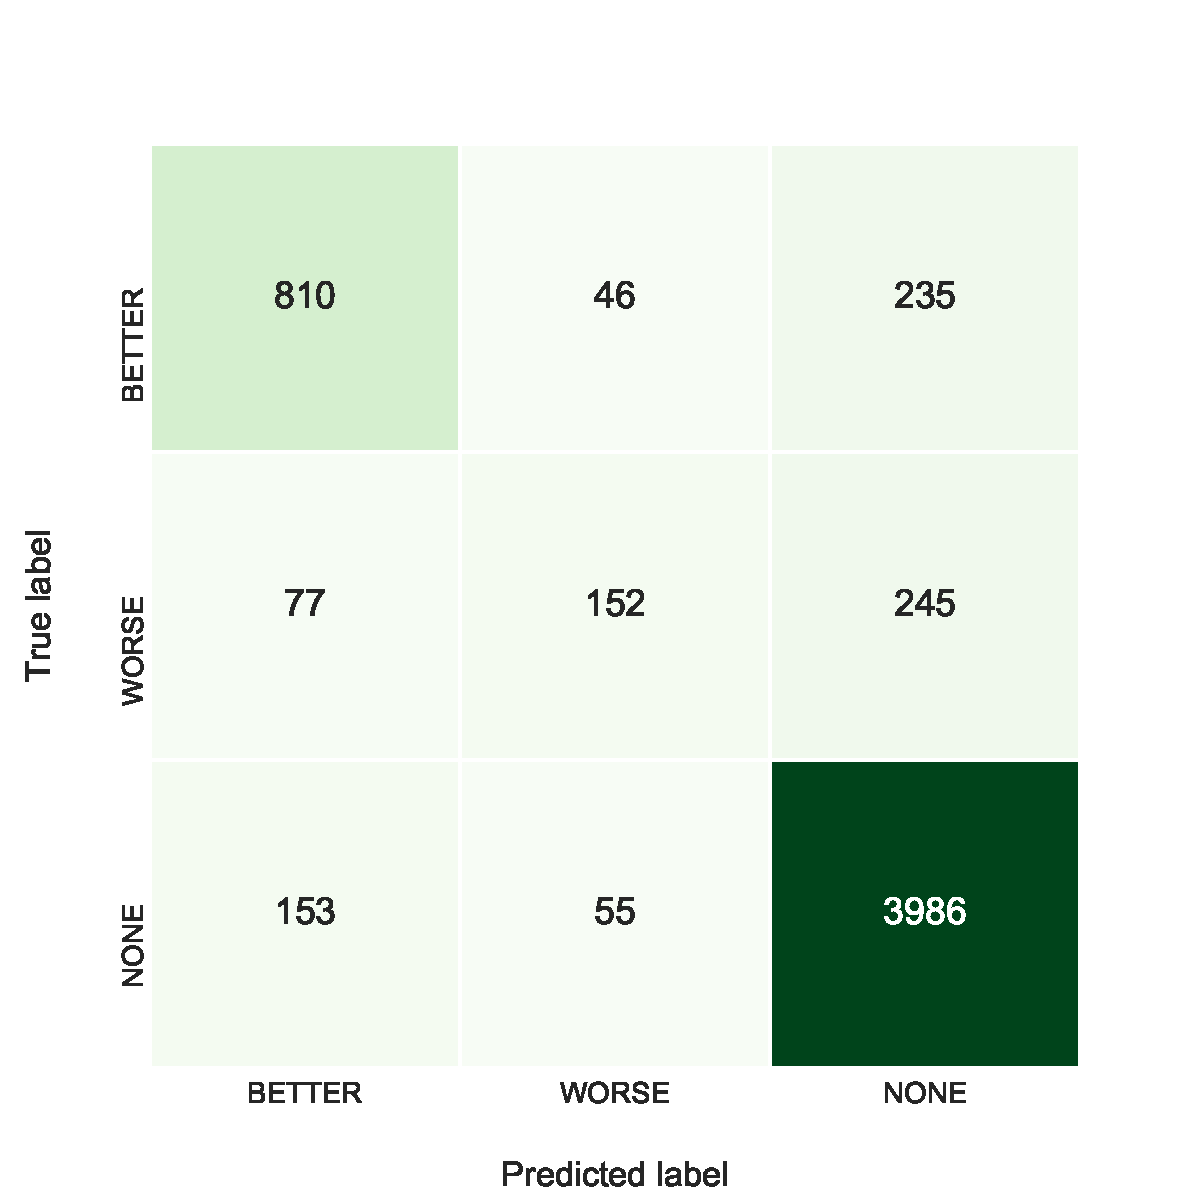
\includegraphics[width=1\linewidth]{images/experiments/conf-InferSent_False}
  \end{minipage} \hfill
    \begin{minipage}{.5\linewidth}
  
     \caption{Confusion matrix for the unigram feature} 
       \label{tbl:3_conf_uni}
 \centering
	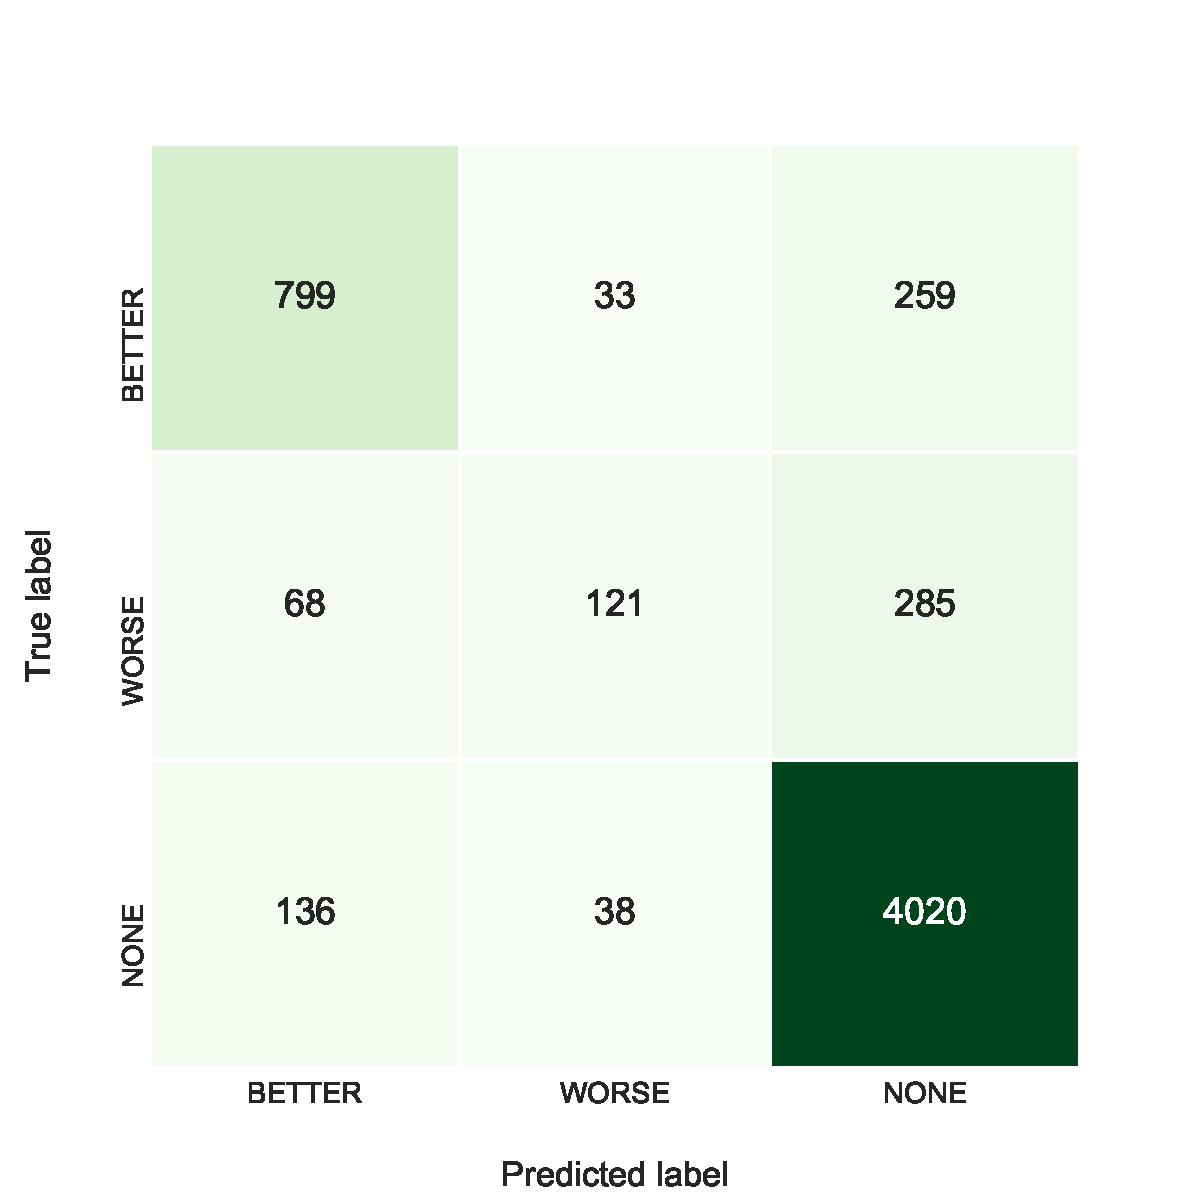
\includegraphics[width=1\linewidth]{images/experiments/conf-Unigrams_False}
    \end{minipage} 
\end{figure}


%\begin{table}[h]
%    \begin{minipage}{.5\linewidth}
%   \caption{Confusion matrix for the sentence embedding feature} 
%    \label{tbl:3_conf_inf}
%
%\begin{tabular}{@{}lrrr@{}}
%\toprule
%       & \texttt{BETTER} & \texttt{WORSE} & \texttt{NONE} \\ \midrule
%\texttt{BETTER} & 832       &  41     &  229    \\
%\texttt{WORSE}  &    97    &    144   &     237 \\
%\texttt{NONE}   &    169    &    52   &    4019  \\ \bottomrule
%\end{tabular}
%
%
%  \end{minipage} \hfill
%    \begin{minipage}{.5\linewidth}
%  
%     \caption{Confusion matrix for the unigram feature} 
%       \label{tbl:3_conf_uni}
%
%\begin{tabular}{@{}lrrr@{}}
%\toprule
%       & \texttt{BETTER} & \texttt{WORSE} & \texttt{NONE} \\ \midrule
%\texttt{BETTER} & 809    &   30    &   263   \\
%\texttt{WORSE}  & 81     &   114    &    283  \\
%\texttt{NONE}   & 139       &   39    &  4062    \\ \bottomrule
%\end{tabular}
%
%    \end{minipage} 
%\end{table}

As presented above, \texttt{WORSE} was the hardest class to recognize. The matrices show that it was more often confused with \texttt{NONE} than with \texttt{BETTER}. This is contrary to the expections. \texttt{BETTER} and \texttt{WORSE} both represent argumentative sentences and it was expected that the distinction between argumentative and not-argumentative is clearer. 

Both features made the same errors on 661 sentences. The unigram model made another 174 errors on sentences which were correctly predicted by the sentence embedding model. The sentence embedding model made 164 unique errors. However, there is no clear pattern which sentences are hard for the unigram or sentence embedding feature. One-hundred-and-fifty wrongly predicted sentences were analysed, examples are shown in table \ref{tbl:3_mistakes}. 

\begin{table}[h]
\caption{Example sentences for errors made by the classifier in the three-label scenario. The objects of interest are printed \textbf{bold}, the assumed error source in \emph{italics}.}
\label{tbl:3_mistakes}
\begin{tabularx}{\linewidth}{lXrr}
\toprule
 & Sentence & Predicted & Gold \\ \midrule
1 & Is a \textbf{BMW}/Benz 5x better than a \textbf{Honda} Civic\emph{?} & \texttt{BETTER} & \texttt{NONE} \\
2 & Will \textbf{google} Music Become Bigger and Better than \textbf{itunes}\emph{?}& \texttt{BETTER} & \texttt{NONE} \\

3 & Apparently the \textbf{wii} \emph{isn't} superior to the \textbf{ds} for Square-enix. & \texttt{BETTER} & \texttt{WORSE} \\
4 & We usually \emph{don't} like \textbf{Microsoft}, but I \emph{don't} think they are worse than \textbf{Google}. & \texttt{WORSE} & \texttt{BETTER} \\

5 & \emph{Worse} than \textbf{coffee}, the effect \textbf{beer} has on my bladder. & \texttt{NONE} & \texttt{BETTER} \\
6 & We obviously linked to \textbf{youtube} above even though \textbf{hulu} has \emph{superior} quality and content.  & \texttt{NONE} & \texttt{WORSE} \\

7 & \textbf{Perl} is \emph{slower} and \emph{faster} than \textbf{Java} & \texttt{WORSE} & \texttt{BETTER} \\

8 & \emph{Goodnight} \textbf{NetBeans}, \emph{Hello} \textbf{Eclipse} & \texttt{NONE} & \texttt{WORSE} \\

9 & A \emph{5-2-1} \textbf{california} team went down, \emph{27-7}, then \emph{5-1-1} \textbf{oregon} fell harder, \emph{33-0}. & \texttt{NONE} & \texttt{BETTER} \\

10 & Remember, you're the one that said the \ textbf{wii} was the \emph{better} Mercedez and the \textbf{ps3} was the \emph{worse} KIA. & \texttt{NONE} & \texttt{BETTER} \\


\bottomrule
\end{tabularx}

\end{table}

As said in the guidelines, all questions should be labelled as \texttt{NONE}. This restriction was hard even for the annotators. Twenty of the 150 sentences were questions, fourteen with \texttt{NONE} as the gold label. Thus, the annotators did not assign the correct label for the remaining six sentences. The label \texttt{BETTER} was predicted for all fourteen sentences with the gold label \texttt{NONE} (sentence one in two in table  \ref{tbl:3_mistakes}).

Twenty sentences contained at least one negation. Sentence three  is a good example for that case. The negation \enquote{\emph{isn't}} changes the meaning of the sentence. If the negation was removed, the classifier would have predicted correctly.


Another error source is the position of the cue word. It is more likely that \texttt{NONE} is predicted if the cue word is not between the two objects. This is due to the fact that the features only look at the words in between the two objects. However, adding information on the position of the cue word did not help to increase the result. % check

The majority of the 150 sentences was just hard to classify. Sentence seven does not have a clear winner; even the human annotators did not assign the correct label (\texttt{NONE}). A lot more training data is needed to enable a classifier to learn that sentence eight is comparative. Same is true for sentence nine, which would also need some knowledge to understand that the numbers are important for the comparison.\newline \newline 


% === binary

Tables \ref{tbl:2_conf_inf} and \ref{tbl:2_conf_uni} show the confusion matrices for the binary setup. Similar to the three-classes scenario, both feature setups made the same mistakes on 517 sentences. The unigram feature produced 204 unique errors, the sentence embeddings 192. It bears mentioning that 765 of the 913 errors are also present in the three-label scenario, so only 148 errors are new. 

\begin{figure}[h]
    \begin{minipage}{.5\linewidth}
   \caption{Confusion matrix for the sentence embedding feature} 
    \label{tbl:3_conf_inf}
 \centering
	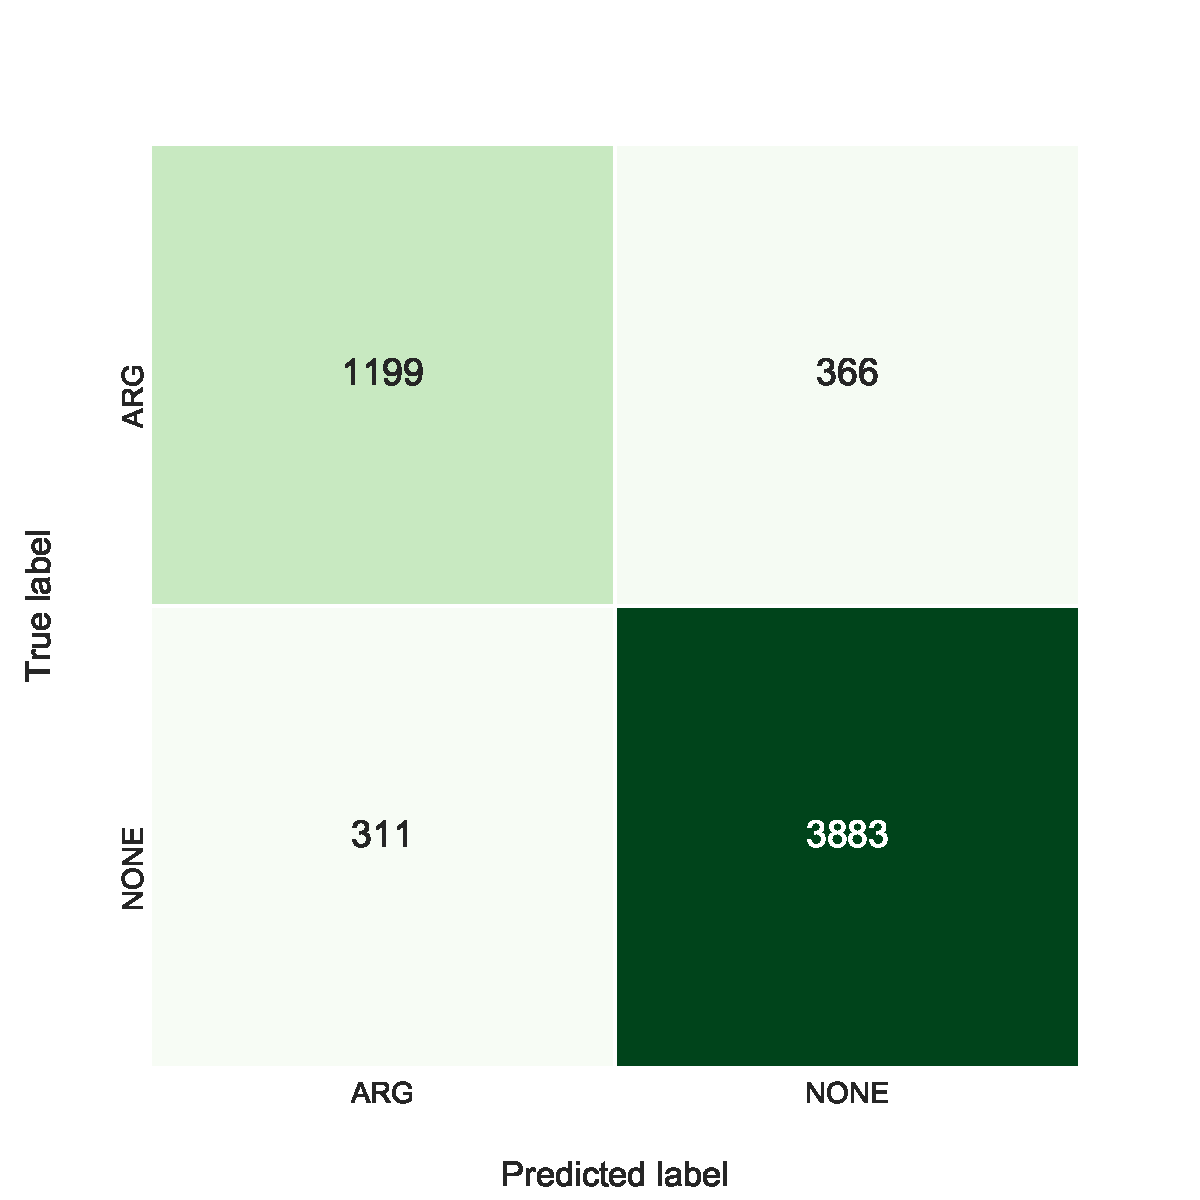
\includegraphics[width=1\textwidth]{images/experiments/conf-InferSent_True}
  \end{minipage} \hfill
    \begin{minipage}{.5\linewidth}
  
     \caption{Confusion matrix for the unigram feature} 
       \label{tbl:3_conf_uni}
 \centering
	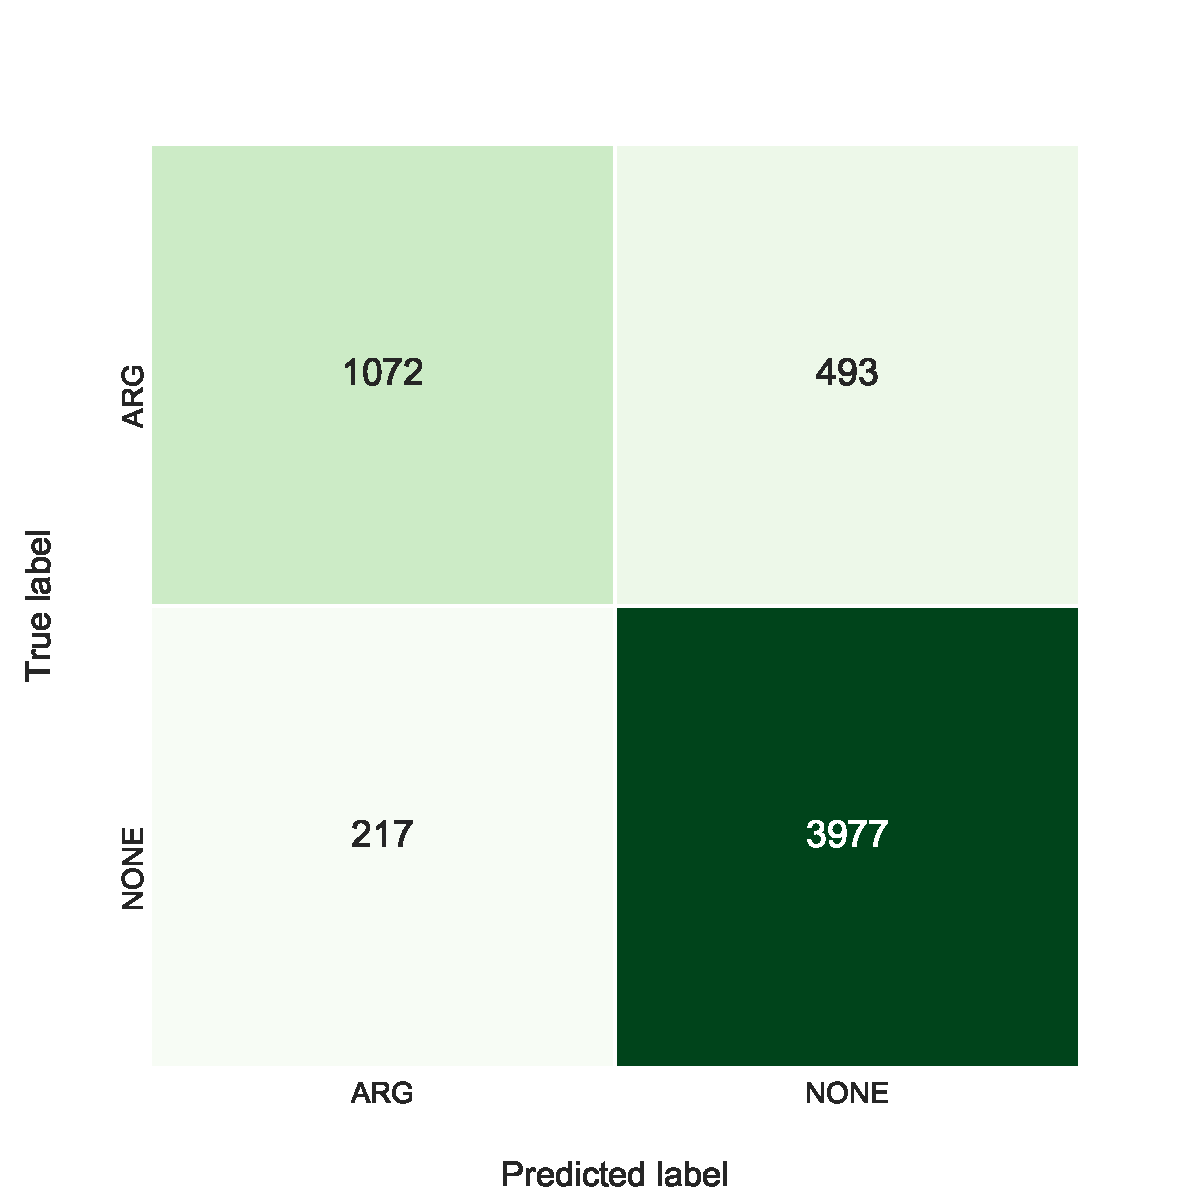
\includegraphics[width=1\textwidth]{images/experiments/conf-Unigrams_True}
    \end{minipage} 
\end{figure}


%\begin{table}[h]
%    \begin{minipage}{.5\linewidth}
%    \centering
%   \caption{Confusion matrix for the sentence embedding feature} 
%    \label{tbl:2_conf_inf}
%
%\begin{tabular}{@{}lrrr@{}}
%\toprule
%       & \texttt{ARG}  & \texttt{NONE} \\ \midrule
%\texttt{ARG} & 1185      &   395   \\
%\texttt{NONE}   & 314          &  3926    \\ \bottomrule
%\end{tabular}
%
%  \end{minipage} \hfill
%    \begin{minipage}{.5\linewidth}
%   \centering
%     \caption{Confusion matrix for the unigram feature} 
%       \label{tbl:2_conf_uni}
%
%\begin{tabular}{@{}lrrr@{}}
%\toprule
%       & \texttt{ARG}  & \texttt{NONE} \\ \midrule
%\texttt{ARG} & 1087      &   493   \\
%\texttt{NONE}   & 228          &  4012    \\ \bottomrule
%\end{tabular}
%
%    \end{minipage} 
%\end{table}

The binary scenario benefits from the reduced class imbalance, yet the errors made are essentially the same. Table \ref{tbl:2_mistakes} shows some example sentences from the 148 new errors.

\begin{table}[h]
\caption{Example sentences for errors made by the classifier in the binary scenario. The objects of interest are printed \textbf{bold}, the assumed error source in \emph{italics}.}
\label{tbl:2_mistakes}
\begin{tabularx}{\linewidth}{lXrr}
\toprule
 & Sentence & Predicted & Gold \\ \midrule
1 & Why \emph{can't} \textbf{Ford} puts better handling into the FWD Fusion if \textbf{Honda} can do it 10 years ago\emph{?} & \texttt{ARG} & \texttt{NONE}\\
2 & \textbf{Java} \emph{isn't} too bad of a first language, but \textbf{Python} is a little easier to pick up. & \texttt{NONE} & \texttt{ARG} \\
3 & My minestrone \textbf{soup} is always better \emph{with} homemade \textbf{pasta}. & \texttt{ARG} & \texttt{NONE} \\
4 & \textbf{Scala} probably embraces \textbf{Java} \emph{better} than any other language in the book. & \texttt{ARG} & \texttt{NONE} \\
5 & \textbf{Windows 8} has efficiency improvements over \textbf{Windows 7}, making it about \emph{10\% faster} overall. & \texttt{NONE} & \texttt{ARG} \\
\bottomrule
\end{tabularx}

\end{table}

The first sentence is an example for the problems with questions and, like the second, negations. In fourth and fifth sentence, the cue word appears after the objects.

\section{Discussion}
The results show that the part between the two objects of interest is most valuable. Also, the objects are not important at all for the classification. Removing or replacing the objects from the sentence did not decrease any score significantally.

Simple features, like the bag-of-words model yielding results similar to the more complexe sentence embeddings.

\section{Evaluation with the held-out data}
\label{sec:final}

